%%%------------------------------------------------------------------------------------------------------------
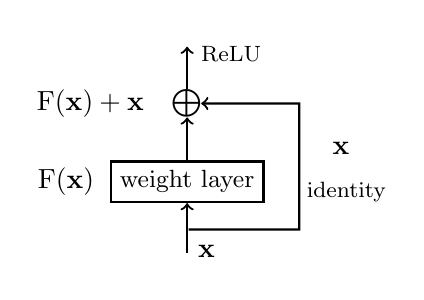
\begin{tikzpicture}
\begin{scope}


\node [anchor=center] (node6) at (0,0) {};
\node[anchor=west](node6-1) at ([xshift=-0.2em,yshift=-0.6em]node6.east) {\footnotesize{$\rm{ReLU}$}};
\node [anchor=north](node3)at ([yshift=-1.2em]node6.south){$\bigoplus$};
\draw[->,thick]([yshift=-0.32em]node3.north)--(node6.south);

\node [anchor=north,draw,thick](node2)at ([yshift=-1.2em]node3.south){\small{weight layer}};
\draw[->,thick](node2.north)--([yshift=0.35em]node3.south);
\node[anchor=west](node2-1) at ([xshift=2.1em,yshift=1.2em]node2.east) {$\mathbf{x}$};
\node[anchor=north](node2-2) at ([xshift=0.2em,yshift=-0.3em]node2-1.south) {\footnotesize{$\rm{identity}$}};

\node [anchor=east](node4) at ([xshift=-0.2em]node2.west) {$\textrm{F}(\mathbf{x})$};
\node [anchor=east](node5) at ([xshift=-0.3em]node3.west) {$\textrm{F}(\mathbf{x})+\mathbf{x}$};

\node [anchor=north](node1) at ([yshift=-1.8em]node2.south) {};
\draw[->,thick]([yshift=0.0em]node1.north)--(node2.south);
\node [anchor=east](node1-1) at ([xshift=1em,yshift=0.4em]node1.east) {$\mathbf{x}$};
\draw[->,thick]([xshift=-1.3em,yshift=0.8em]node1-1.east)--([xshift=2.7em,yshift=0.8em]node1-1.east)--([xshift=2.7em,yshift=5.35em]node1-1.east)--([xshift=-0.4em]node3.east);




\end{scope}
\end{tikzpicture}
%%%------------------------------------------------------------------------------------------------------------






